\chapter{НАСТРОЙКА ПОЛЬЗОВАТЕЛЬСКИХ ДЕМОНОВ SYSTEMD}

\section{Цель работы}
Сконфигурировать пользовательские демоны на базе systemd: написать два bash-скрипта для уведомлений об отдыхе/возврате к работе и настроить их запуск через service+timer. Зафиксировать ход в \texttt{record\_result\_lab\_5}.

\section{Краткий ход выполнения}
\subsection{Подготовка и генерация варианта}
- Запущена запись терминала: \texttt{script -a record\_result\_lab\_5}
- Распакован архив \texttt{faces.tar.gz}, проверено наличие \texttt{lab5.py} и каталога \texttt{images}
- Сгенерирован вариант: \texttt{python lab5.py} (скриншот добавить)

\subsection{Bash-скрипты}
\paragraph{eyes-start.sh} выводит уведомление «Time to relax, senpai!» на период \texttt{repetition\_period} секунд; принимает параметром секунды и переводит их в миллисекунды для \texttt{notify-send}.
\paragraph{eyes-stop.sh} ждёт \texttt{relax\_time} и выводит уведомление «Time to get back to work, senpai!» на 5 секунд.

\subsection{Unit-файлы systemd}
- \texttt{eyes-relax.service}: запускает \texttt{eyes-start.sh} с параметром \texttt{relax\_time}
- \texttt{eyes-relax.timer}: обеспечивает периодичность \texttt{OnUnitActiveSec=repetition\_period}
- \texttt{eyes-stop.service}: запускает \texttt{eyes-stop.sh}, зависит от запуска стартового сервиса

\section{Код и конфигурации}
\subsection{Скрипт eyes-stop.sh}
\begin{lstlisting}[language=bash]
#!/bin/bash

relax_time=$1
sleep "$relax_time"
icon=/home/Desktop/images/icon.png
notify-send -i "$icon" -t 5000 "Time to get back to work, senpai!" "5 seconds"
\end{lstlisting}

\subsection{eyes-relax.service}
\begin{lstlisting}
[Unit]
Description=eye relax daemon
After=eyes-stop.service
Wants=eyes-stop.service

[Service]
Type=simple
Environment="DISPLAY=:0"
Environment="XAUTHORITY=/home/<user>/.Xauthority"
Environment="DBUS_SESSION_BUS_ADDRESS=unix:path=/run/user/1000/bus"
User=<user>
Group=<user>
WorkingDirectory=/home/<user>/Desktop/
ExecStart=/home/<user>/Desktop/eyes-start.sh <relax_time>
\end{lstlisting}

\subsection{eyes-relax.timer}
\begin{lstlisting}
[Unit]
Description=scheduler for eyes service

[Timer]
OnBootSec=60s
OnUnitActiveSec=<repetition_period>s

[Install]
WantedBy=timers.target graphical.target
\end{lstlisting}

\subsection{eyes-stop.service}
\begin{lstlisting}
[Unit]
Description=eye stop relax daemon
Requires=eyes-relax.service

[Service]
Type=simple
Environment="DISPLAY=:0"
Environment="XAUTHORITY=/home/<user>/.Xauthority"
Environment="DBUS_SESSION_BUS_ADDRESS=unix:path=/run/user/1000/bus"
User=<user>
Group=<user>
WorkingDirectory=/home/<user>/Desktop/
ExecStart=/home/<user>/Desktop/eyes-stop.sh <relax_time>

[Install]
WantedBy=graphical.target
\end{lstlisting}

\section{Команды управления}
- Перечитать юниты: \texttt{sudo systemctl daemon-reload}
- Запуск таймера: \texttt{sudo systemctl start eyes-relax.timer}
- Статусы: \texttt{sudo systemctl status eyes-relax.timer|eyes-relax.service|eyes-stop.service}
- Автозапуск: \texttt{sudo systemctl enable eyes-relax.timer}
- Остановка/отключение: \texttt{sudo systemctl stop|disable eyes-relax.timer}


\section{Вывод}
Настроены пользовательские демоны systemd: единичный сервис для старта уведомлений, зависимый сервис для уведомления окончания и таймер, обеспечивающий периодический запуск. Управление производится через \texttt{systemctl}, логирование доступно через \texttt{journalctl}.

% Results screenshots
\section{Скриншоты результатов}
\begin{figure}[H]
  \centering
  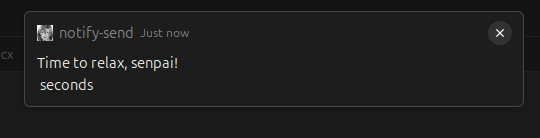
\includegraphics[width=0.95\textwidth]{results/image1.png}
  \caption{Уведомление начала отдыха}
\end{figure}
\begin{figure}[H]
  \centering
  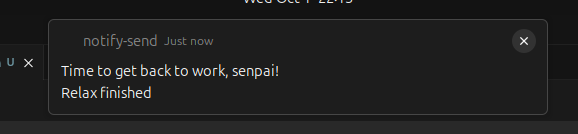
\includegraphics[width=0.95\textwidth]{results/image3.png}
  \caption{Уведомление окончания отдыха}
\end{figure}
\begin{figure}[H]
  \centering
  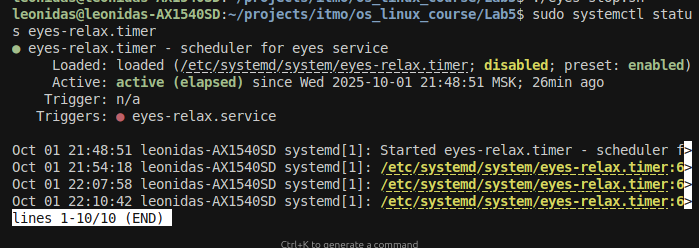
\includegraphics[width=0.95\textwidth]{results/status1.png}
  \caption{Статус юнитов (таймер/сервисы) 1}
\end{figure}
\begin{figure}[H]
  \centering
  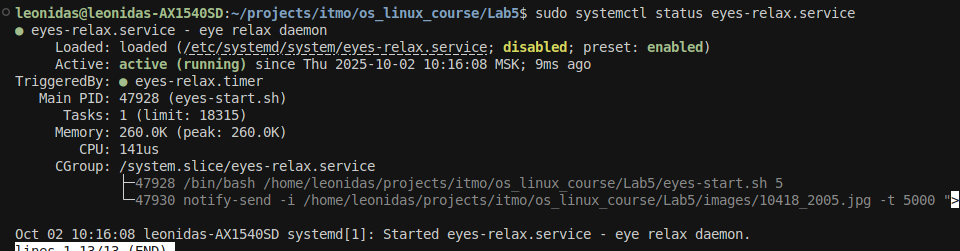
\includegraphics[width=0.95\textwidth]{results/status2.png}
  \caption{Статус юнитов 2}
\end{figure}
\begin{figure}[H]
  \centering
  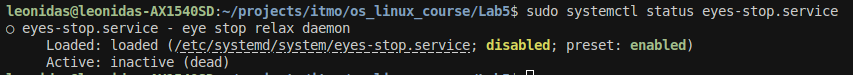
\includegraphics[width=0.95\textwidth]{results/status3.png}
  \caption{Статус юнитов 3}
\end{figure}
